\section*{Exercise 4}
\subsection*{rep-24}
The full command we used for retrieving the \textit{csv} file is listed in figure \ref{fig:bash-flowrec}.
\begin{figure}[H]
\begin{lstlisting}[language=bash]
rwcut --num-recs=200000 --delimited=',' --fields=sIP,dIP,sPort,dPort,protocol,flags,ttl,bytes team16.flowrecord.rw > team16_flowrecord.csv
\end{lstlisting}
\caption{ Bash command for retrieving the flow record csv file }
\label{fig:bash-flowrec}
\end{figure}
\subsection*{rep-25}
\begin{table}[H]
\center
\begin{tabular}{lr}
\toprule
port & count \\
\midrule
80 & 31022 \\
0 & 7357 \\
29001 & 1890 \\ 
\bottomrule
\end{tabular}
\caption{ The three most frequent source ports }
\label{tab:most-frequent-source-ports}
\end{table}

\begin{table}[H]
\center
\begin{tabular}{lr}
\toprule
port & count \\
\midrule
445 & 79793 \\
10320 & 32014 \\
3389 & 7834 \\
\bottomrule
\end{tabular}
\caption{ The three most frequent destination ports }
\label{tab:most-frequent-destination-ports}
\end{table}

\begin{table}[H]
\center
\begin{tabular}{lr}
\toprule
protocol & rate \\
\midrule
6 (TCP) & 72.9165\% \\
17 (UDP) & 23.462\% \\
1 (ICMP) & 3.5845\% \\
41 (IPv6) & 0.0365\% \\
47 (GRE) & 0.0005\% \\
\bottomrule
\end{tabular}
\caption{ Frequency of protocols }
\label{tab:all-protocols}
\end{table}

\subsection*{rep-26}
One remarkable finding was, that there are no common used ports under the most occurring destination ports.
By looking at the histograms for source IP addresses we found out that a small number of addresses sent most packages. The same applies to the histogram of destination IP addresses.

\subsection*{rep-27}

\begin{figure}[H]
\center
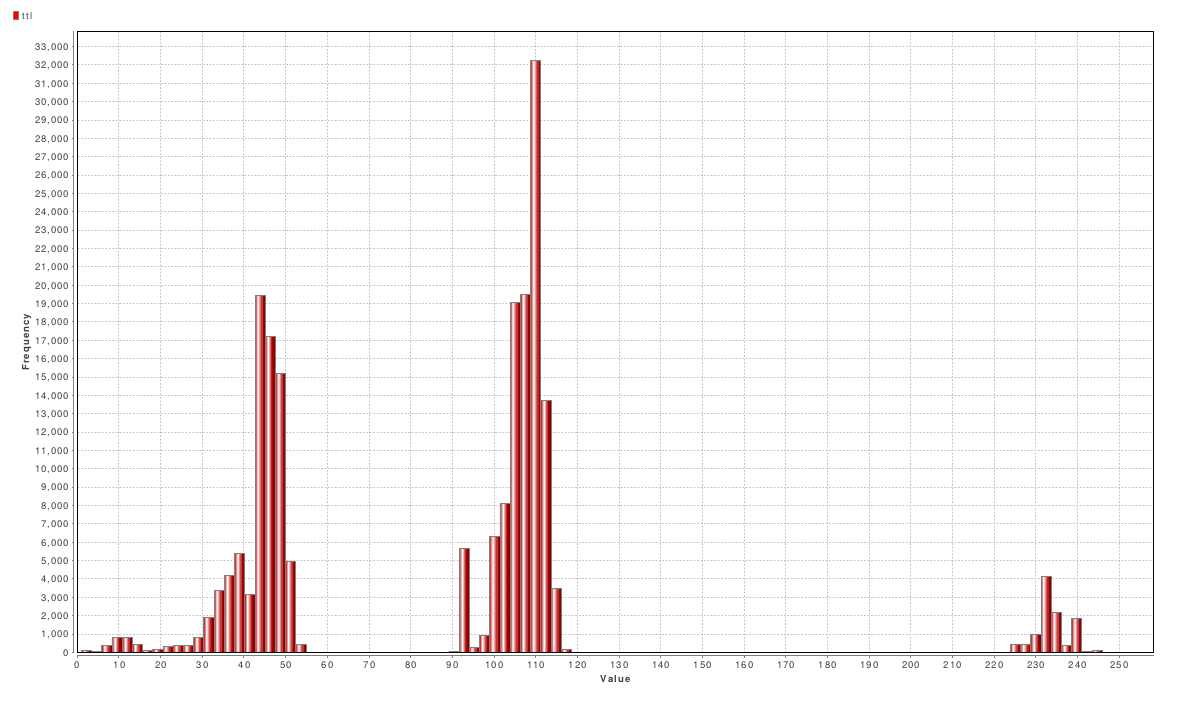
\includegraphics[width=0.7\textwidth]{./chapters/plots/rep-27-ttl}\\
\caption{TTL distribution of packets}
\label{fig:ttl-distribution}
\end{figure}

There seem to be standard values for TTL around 45, 110 and 230. Although they should be standardized there are some slight deviations from them.

\subsection*{rep-28}
The most recurring IP source address is \textbf{85.167.14.252}.
It is easy to find (e.g. by looking at the bytes histogram (figure \ref{fig:bytes-histo}) out that all packets this host sent were of the same size. In addition this host accessed a wide range of IP addresses and a wide range of ports. Additionally that this IP tries to connect to two random ports on a destination address. Therefore we can conclude, that this IP tries to do a horizontal scan, whereby each destination is probed on two random ports.

\begin{figure}[H]
\center
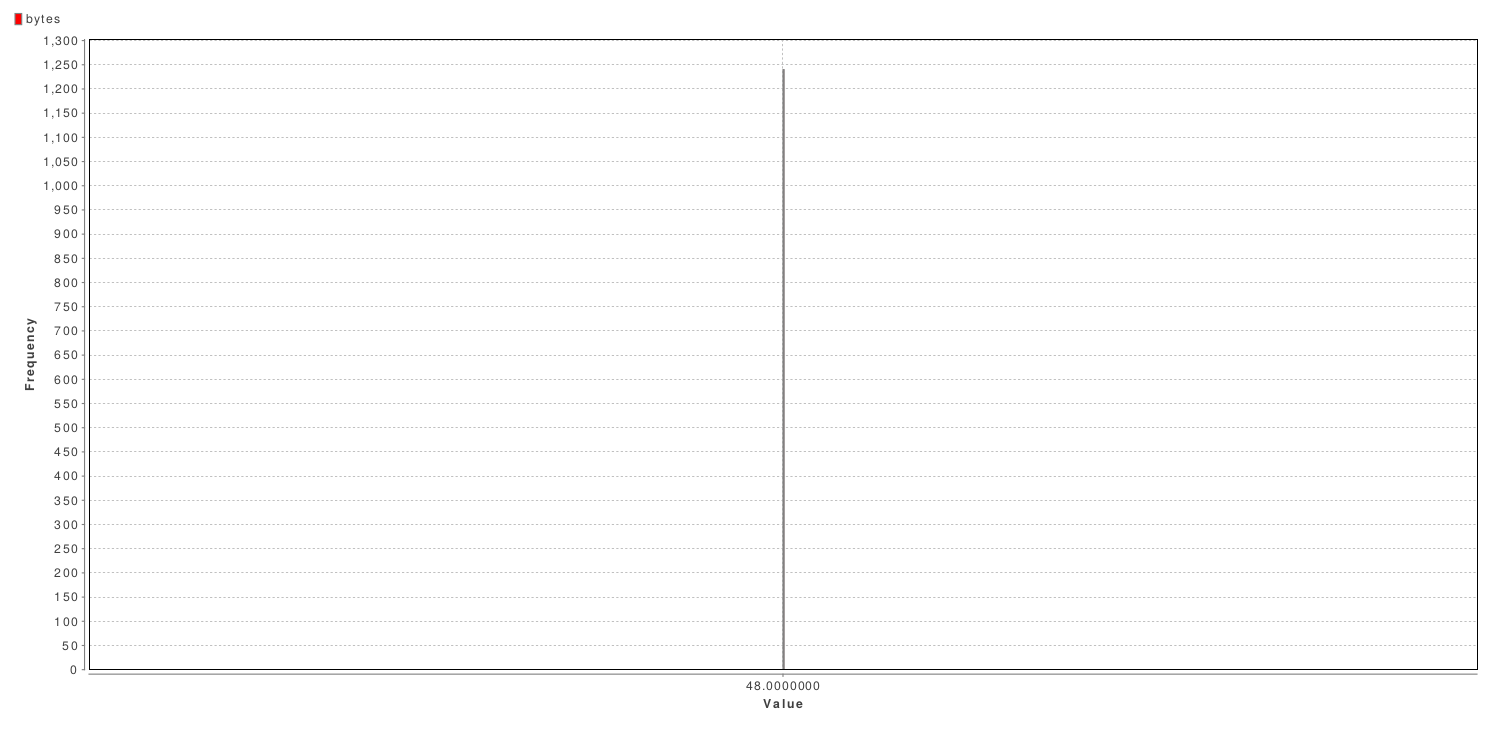
\includegraphics[width=.7\textwidth]{./chapters/plots/rep-28-bytes-histo}\\
\caption{bytes histogramm of all packets sent by 88.167.14.252}
\label{fig:bytes-histo}
\end{figure}

\subsection*{rep-29}
The source IP address, that connected to highest number of destination Ports is again the source IP address \textbf{85.167.14.252}. This is the same IP address as in \textit{rep-28}. Hence it's has the same behavior.

\begin{figure}[H]
\center
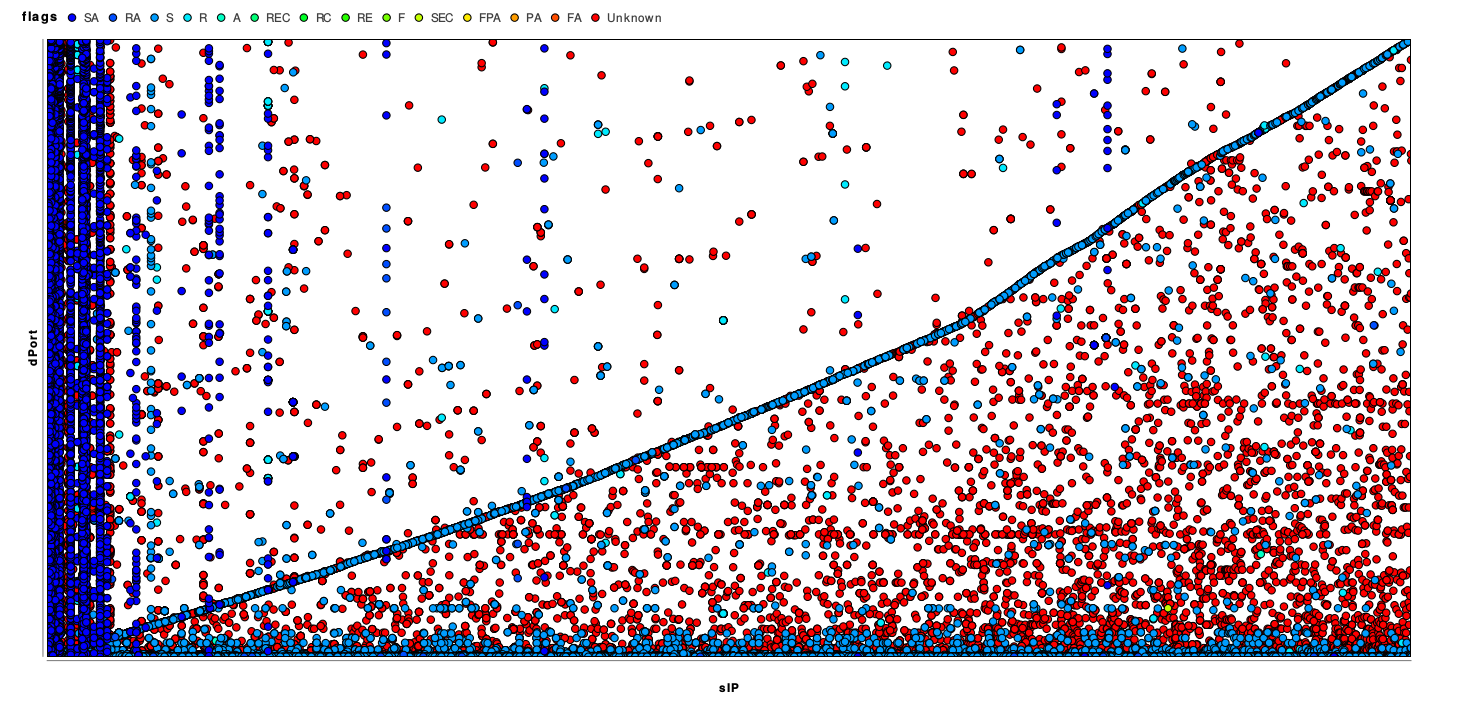
\includegraphics[width=.7\textwidth]{./chapters/plots/rep29.png}\\
\caption{Scatter Plot sIP - dPort}
\end{figure}

\subsection*{rep-30}
The port, that is getting the most connections from different IP sources is the port 445. It is getting IP connections from 79793 different IP sources. It receives the biggest amount of packets from the source IP \textbf{190.253.254.250} (1240 packets). \\

\lstinputlisting[label={lst:rapidminer_experiment},
				caption=Rapidminer experiment setup, language=XML]
				{./chapters/rapidminer/experiment.xml}

Port 445 is the SMB Port on Microsoft Windows machines. It is known, that this port has a vulnerability, that is exploited by the NetBIOS worm. After a machine is infected, it performs further scan attempts. In our case the machine \textbf{190.253.254.250} only sends packets to a very small number of different IP addresses. Either this is client with a bad configuration, that tries to connect to this IP address.

